\chapter{Theoretical Motivations
\label{ch:theory}}

\setcounter{section}{-1}

\section{The Standard Model}

The standard model (SM) of particle physics includes three fundamental forces and all of the particles of ordinary matter using a quantum field theory framework. When forces are weak enough, quantum field theory calculations use a perturbative method in which the leading order (LO) term is calculated, then the next-to-leading order (NLO) correction is added, then the next-to-next-to-leading order correction (NNLO), and so forth. The three fundamental forces are electromagnetism, the weak force, and the strong force. These forces are carried by spin-1 gauge bosons, while the matter particles consist of quarks and leptons, two categories of spin-1/2 fermions. In addition, the standard model contains a scalar spin-0 boson, the Higgs boson, which is part of the Higgs field that provides masses to certain gauge bosons and fermions. Figure \ref{fig:sm-particles} summarizes the particles in the standard model, including the spin, electric charge, and mass values of each particle. The standard model and quantum field theory are described in more detail in \cite{Griffiths} and \cite{Peskin}.

\begin{figure}[hbt]
\begin{center}
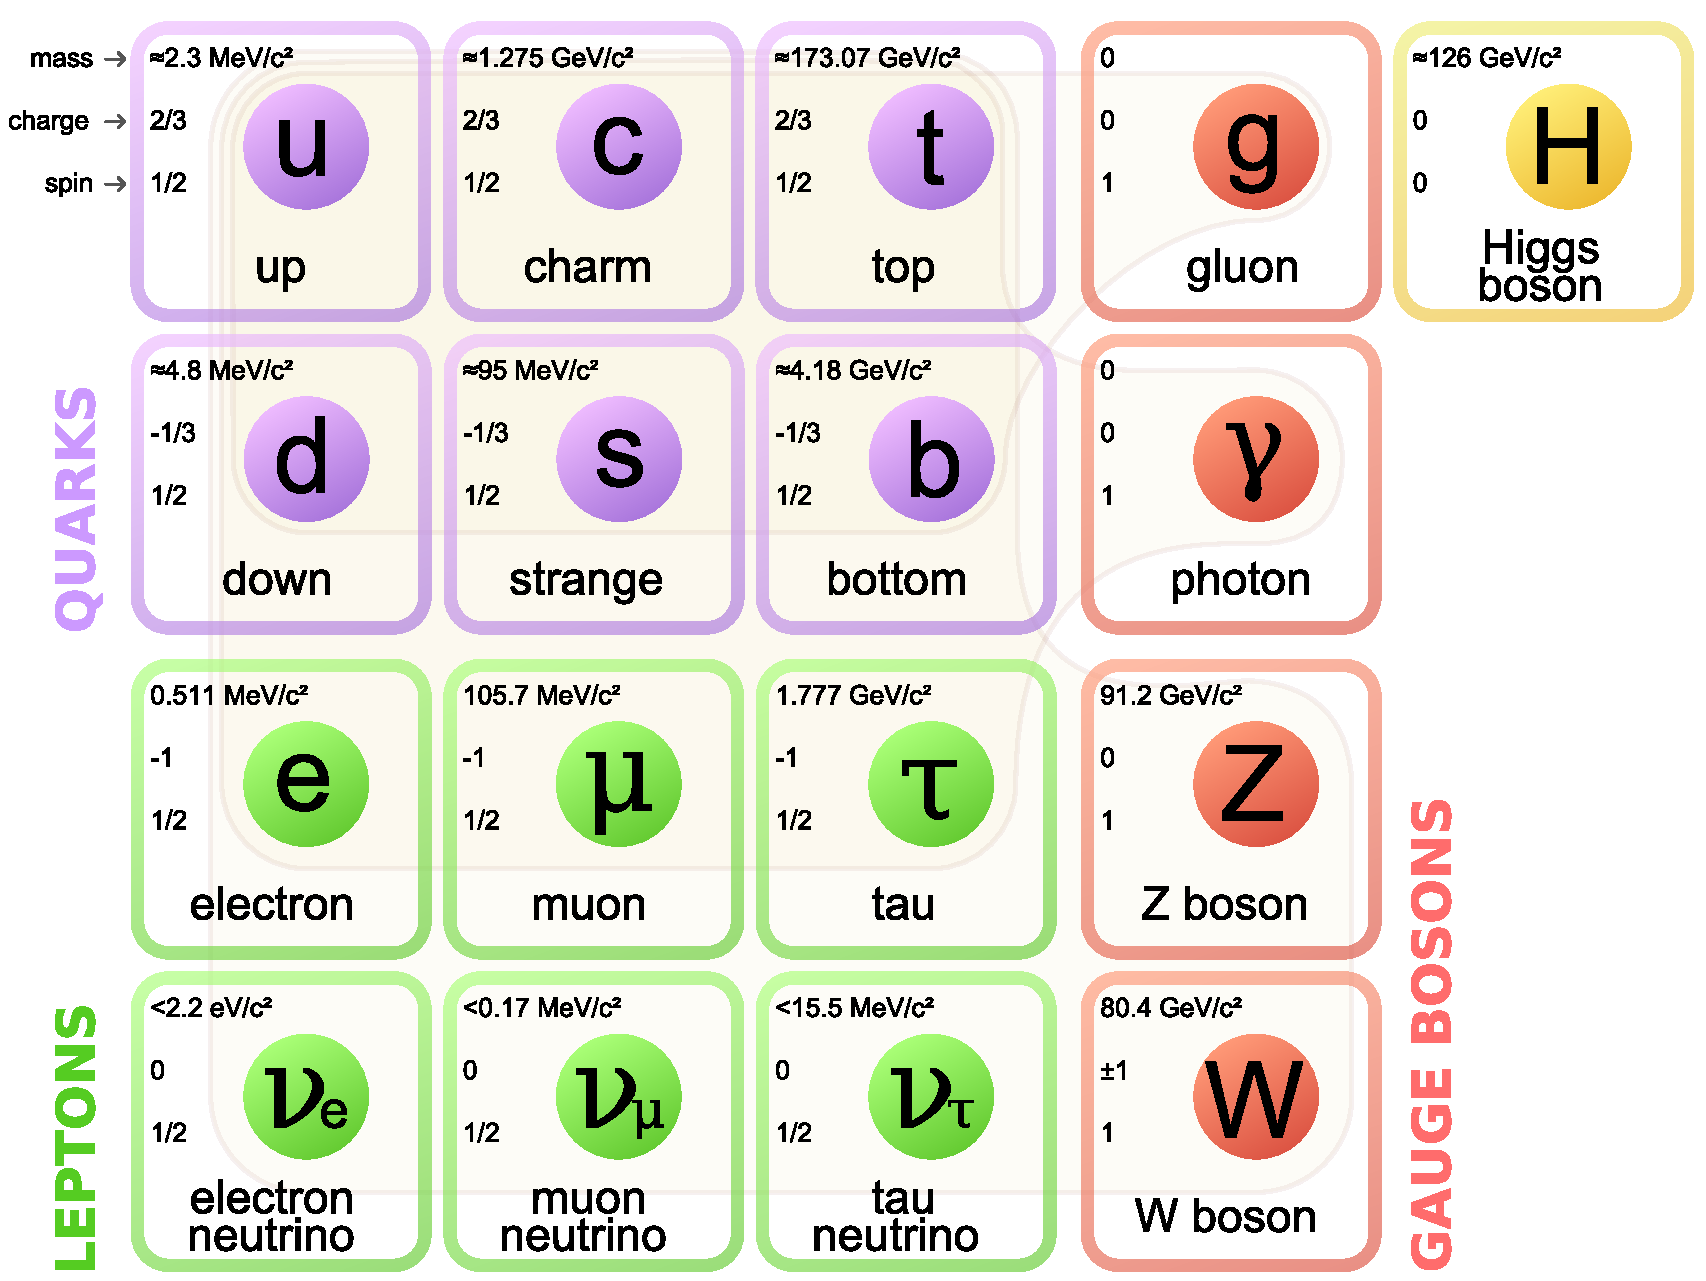
\includegraphics[width=0.95\textwidth]{figures/Standard_Model_of_Elementary_Particles.pdf}
\caption{A table of all the elementary particles in the standard model, with the spin, electric charge, and mass values of each particle \cite{MissMJ}. The faint gray lines indicate which gauge bosons interact with which fermions.}
\label{fig:sm-particles}
\end{center}
\end{figure}

The electromagnetic force is mediated by photons ($\gamma$), spin-1 gauge bosons which have no mass or electric charge $Q$. This force causes interactions between electrically charged particles and has infinite range due to the masslessness of the photon. Quantum electrodynamics (QED) is the quantum field theory description of electromagnetism, which can be represented by a $U(1)$ symmetry group. The weak force is mediated by the massive \Wpm and \Z bosons and can be represented by an $SU(2)$ symmetry group. The weak force acts on particles carrying weak isospin $T$. Weak isospin is a quantum number whose third component $T_3$ is conserved in all interactions and which can be mathematically treated in the same way as angular momentum, though the two quantities are physically distinct. The massiveness of the weak carrier bosons means that the weak force has a limited range, approximately $10^{-18}\unit{m}$. The charged current weak interaction, mediated by the \Wpm bosons, is sensitive to the chirality of fermions; only left-handed fermions and right-handed antifermions participate in this interaction. The neutral current weak interaction, mediated by the \Z boson, is not sensitive to chirality.

As suggested by the inclusion of both forces in the previous paragraph, the electromagnetic and weak forces can be unified to form the electroweak force, represented by the symmetry group $SU(2) \times U(1)$. In this unification, the quantum numbers of electromagnetism and the weak force are related by a new conserved quantum number, weak hypercharge $Y = 2(Q - T_3)$. The Higgs mechanism is responsible for electroweak symmetry breaking (EWSB). In order for the electroweak theory to be gauge invariant, the gauge bosons must be massless, but the \Wpm and \Z bosons are observed to have mass. The Higgs mechanism solves this dilemma via spontaneous EWSB due to its non-zero vacuum expectation value (VEV). The Higgs field consists of a doublet, with two charged particles and two neutral particles, all scalar bosons. The two charged particles and one of the neutral particles act as Goldstone bosons, combining with the \Wpm and \Z bosons to produce their masses. The remaining neutral particle is the Higgs boson, which was discovered at the LHC in 2012 \cite{NewBoson}.

The strong force, quantum chromodynamics (QCD), is mediated by gluons (\cPg) and can be represented by an $SU(3)$ symmetry group. Gluons, like photons, are spin-1 gauge bosons without mass or electric charge. However, gluons do possess color charge, the quantum number on which the strong force acts. Color charge is so named because the charge has three possible values, which are labeled red, green, or blue. Because gluons both mediate and participate in the strong interaction, the force between quarks does not decrease as they become spatially separated. The energy in the gluon field between the separated quarks can become large enough to form one or more quark-antiquark pairs. This phenomenon is known as confinement and prevents quarks or gluons from existing in a bare state. Correspondingly, the range of the strong force is limited to ${\sim} 10^{-15}\unit{m}$. Bound states of quarks and gluons, the only way they have ever been observed in nature, are called hadrons, and the formation of those bound states is called hadronization. States with one quark and one antiquark are mesons, while states with three quarks are baryons. Mesons and baryons are the two allowed types of bound states because they represent color singlets. Complementarily, as quarks get closer together, the strong force between them weakens. This behavior is known as asymptotic freedom; because short distances are equivalent to high energies, the strong interactions of quarks at a high-energy collider like the LHC can be calculated perturbatively. A residual form of the strong force acts on nucleons, protons and neutrons, to form atomic nuclei.

As mentioned, fermions are the particles of matter, which are separated into two groups: quarks and leptons. Quarks have fractional electric charge, weak isospin, and color charge, so they are affected by all three fundamental forces. There are two types of quarks: up-type quarks that have $Q = 2/3$ and down-type quarks that have $Q = -1/3$. Leptons consist of charged leptons and neutrinos. Charged leptons possess electric charge and weak isospin, while neutrinos only possess weak isospin. Three generations exist for each type of particle, with the different particles called flavors. The flavors of up-type quarks are the up, charm, and top quarks; of down-type quarks are the down, strange, and bottom quarks; of charged leptons are the electron, muon, and tau lepton; and of the neutrinos are the electron, muon, and tau neutrinos. The charged current weak interaction mixes the different flavors of quarks, with the amount of mixing between any two flavors given by the unitary Cabibbo-Kobayashi-Maskawa (CKM) matrix. The top quark is the heaviest elementary particle and is so heavy that it decays before hadronizing, making it an exception to the rule that bare quarks are not observed. Quarks possess an additively conserved quantum number called baryon number $B$, which is defined as $B = \frac{1}{3}(n_{\cPq} - n_{\overline{\cPq}})$. Similarly, lepton number $L$ is defined for leptons as $L = n_{\ell} - n_{\overline{\ell}}$. Specific lepton flavor numbers $L_{\Pe}$, $L_{\mu}$, $L_{\tau}$ are defined for each flavor pair of leptons.

The fermions are arranged into multiplets based on their chirality. The left-handed up- and down-type quarks are grouped together in a doublet $\cPq_L$, as are the left-handed charged leptons and neutrinos in $\ell_L$. The right-handed particles are singlets. It is important to note that right-handed neutrinos, and correspondingly left-handed antineutrinos, do not exist in the standard model. The Higgs field spontaneously provides masses to the quarks and charged leptons through a Yukawa interaction which couples the left- and right-handed versions of each flavor of particle. The quantum numbers of each type of particle are summarized in Table \ref{tab:q-num}, and the interactions among all the particles are illustrated in Fig. \ref{fig:sm-interactions}.

\begin{table}[htb]
  \begin{center}
    \def\arraystretch{2.0} %1 is the default
    \begin{tabular}{|l||l|c|c|c|c|c|}
\hline
      & Particle & $Q$ & $T_3$ & $Y$ & $B$ & $L$ \\
\hline
\hline
\multirow{3}{*}{Quarks}  & $\cPq_L = \displaystyle\binom{\cPqu}{\cPqd}_L$ & $\displaystyle\binom{2/3}{-1/3}$ & $\displaystyle\binom{1/2}{-1/2}$ & $1/3$  & $1/3$ & 0 \\
                         & $\cPqu_R$                                      & $2/3$                            & 0                                & $4/3$  & $1/3$ & 0 \\
                         & $\cPqd_R$                                      & $-1/3$                           & 0                                & $-2/3$ & $1/3$ & 0 \\
\hline
\multirow{2}{*}{Leptons} & $\ell_L = \displaystyle\binom{\nu}{\Pe}_L$     & $\displaystyle\binom{0}{-1}$     & $\displaystyle\binom{1/2}{-1/2}$ & $-1$   & 0     & 1 \\
                         & $\Pe_R$                                        & $-1$                             & 0                                & $-2$   & 0     & 1 \\
\hline
    \end{tabular}
    \caption{The quantum numbers of each category of fermions, based on chirality and particle type: up-type quarks, down-type quarks, charged leptons, and neutrinos. The various flavors of each category, also called the first, second, and third generations of matter, possess the same quantum numbers and differ only in their masses.}
    \label{tab:q-num}
  \end{center}
\end{table}

\begin{figure}[hbt]
\begin{center}
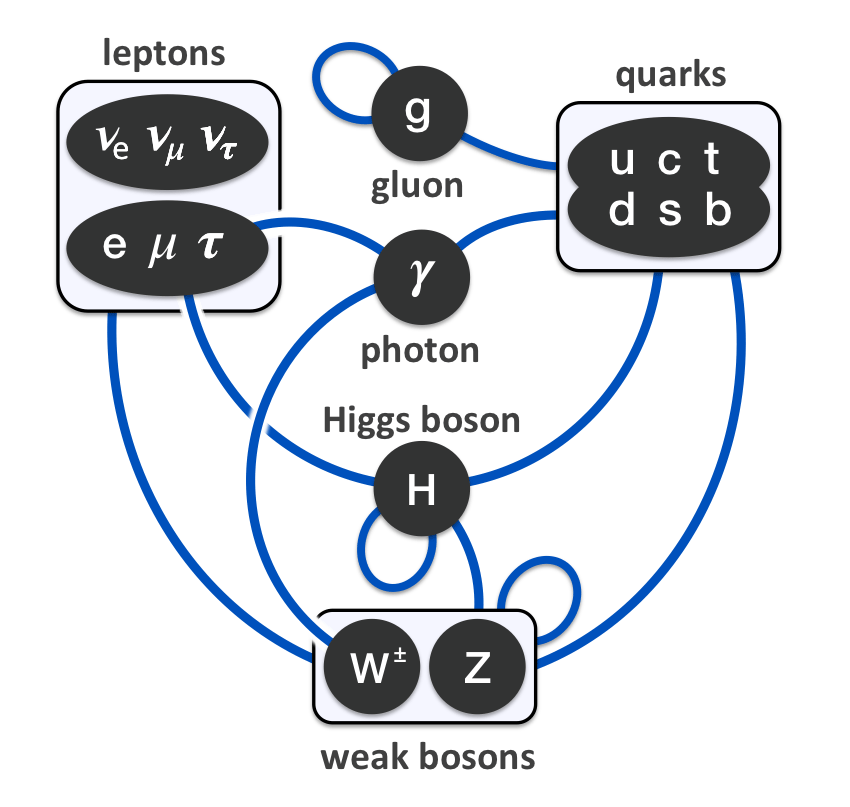
\includegraphics[width=0.95\textwidth]{figures/Elementary_particle_interactions_in_the_Standard_Model.png}
\caption{A diagram illustrating the leading order interactions between particles in the standard model, including self-interactions \cite{Drexler}.}
\label{fig:sm-interactions}
\end{center}
\end{figure}

\addtocounter{section}{-1}
\renewcommand{\thesection}{\thechapter.{$\frac{1}{2}$}}
\section{Beyond the Standard Model}
\renewcommand{\thesection}{\thechapter.\arabic{section}} % back to regular numbering

The predictions of the standard model have been confirmed by decades of precise experimental tests. However, as an effective field theory, its domain of applicability is ultimately limited; at a high enough energy, the theory will break down. Further, the standard model is unable to account for some observations. These limitations and indications of new phenomena motivate various searches for physics beyond the standard model (BSM), include the searches which will be presented in this analysis.

The most obvious limitation of the standard model is that it depends on 19 free parameters which must be determined by experiment. These parameters include the 9 fermion masses, the Higgs mass and VEV, the gauge couplings for the three forces, the three mixing angles and one phase from the CKM matrix, and finally the QCD vacuum angle. It is conceivable that a BSM theory could reduce the number of free parameters. Electroweak unification and charge quantization suggest that a Grand Unified Theory (GUT) could unify all three fundamental forces, at an expected energy scale of ${\sim} 10^{16}\GeV$. The observation of neutrino oscillations is now well established, indicating that neutrinos have small but non-zero masses. The oscillation of neutrinos between mass and flavor eigenstates is described by the Pontecorvo-Maki-Nakagawa-Sakata (PMNS) matrix. Like the CKM matrix for quarks, the PMNS matrix is unitary and has four parameters: three mixing angles and one phase. The values of the neutrino masses have not been directly measured, but are indirectly limited to the \eVns scale. Because right-handed neutrinos do not exist in the Standard Model, neutrinos cannot gain mass via a Yukawa interaction with the Higgs field. Though the Higgs mass is a parameter of the SM, it can be calculated in many BSM theories. Unless unnatural fine-tuning occurs, the presence of new massive particles makes this calculation produce a value near the Planck scale of $10^{19}\GeV$, orders of magnitude higher than the observed value of 125\GeV, which characterizes the electroweak scale. This is known as the hierarchy problem. To construct a natural theory which avoids such fine-tuning while making predictions that agree with observation, it is necessary to cancel divergent contributions to the Higgs mass. The hierarchy problem is an important motivation to search for new physics at the LHC \cite{Morrissey20121}.

Astrophysics provides numerous indications of the need for BSM theories. Most notably, gravity is not included in the standard model. A successful unification of general relativity and quantum field theory has not been achieved, due to the difficulty of constructing a renormalizable theory for the spin-2 graviton. At the Planck scale, gravitational effects become comparable to SM interactions, which calls for a new theory. The measurement of galactic rotation curves and galaxy cluster collisions \cite{BulletCluster} indicates that ${\sim} 85\%$ of the matter in the universe is dark matter, which interacts gravitationally but not electromagnetically. Dark matter is likely to be a new particle not present in the standard model. The most popular type of dark matter candidate is a weakly interacting massive particle (WIMP) \cite{Morrissey20121}, but many other candidates have been proposed. The dearth of antimatter relative to the amount of matter in the universe requires greater violation of charge-parity (CP) symmetry than is contained in the SM. The accelerating expansion of the universe, observed using standard candle supernovae \cite{Supernova98,Supernova99}, implies that ${\sim} 70\%$ of the energy of the universe exists in a unknown form called dark energy. Dark energy may be due to the cosmological constant of the universe, which can be related to the energy of the vacuum in quantum field theory. However, the standard model predicts that this cosmological constant would be $10^{120}$ times larger than the observed value, a clear failure of the theory. The recent tentative evidence for cosmic inflation from the BICEP experiment \cite{BICEP} implies the existence of the inflaton, a new scalar field.

The following sections discuss the theories of leptoquarks (LQs) and R-parity violating (RPV) supersymmetry (SUSY). Leptoquarks are motivated by grand unification and the parallels between leptons and quarks in the standard model. Numerous theories contain some form of LQs. SUSY is motivated by basic considerations of quantum field theory, the hierarchy problem, grand unification, and dark matter. The introduction of R-parity violation in SUSY evades existing limits on signatures with large missing transverse energy due to the stability of the lightest supersymmetric particle (LSP), while retaining the other desirable characteristics of SUSY. RPV SUSY can also act as a signature generator to suggest novel searches which might discover or rule out other BSM theories \cite{EvansSigGen}.

\section{Leptoquarks}

\section{R-Parity Violating Supersymmetry}